\documentclass[11pt]{article}
\newcommand{\ddd}{September 23, 2023}
\input{23cac-macro}

\begin{document}
\begin{center}
  \textbf{Topic 5: Monotone functions and convex functions}
\end{center}

In this topic we discuss properties on monotone functions and convex functions.
Most properties can be assigned as hard exercises.
Nevertheless we hereby indicate some of these since they can be useful later on.

\begin{defn}
  Let $I$ be an interval in $\mathbb{R}$, and $f$ be a real function defined on $I$.
  \begin{enumerate}[(i)]
    \item $f$ is said to be \textsf{increasing} (resp.\ \textsf{strictly increasing}) on $I$ if $f(x_1) \leqslant f(x_2)$ (resp.\ $f(x_1) < f(x_2)$) whenever $x_1, x_2 \in I$ and $x_1 < x_2$.
  
    \item $f$ is said to be \textsf{decreasing} (resp.\ \textsf{strictly decreasing}) on $I$ if $f(x_1) \geqslant f(x_2)$ (resp.\ $f(x_1) > f(x_2)$) whenever $x_1, x_2 \in I$ and $x_1 < x_2$.
      \item $f$ is said to be \textsf{monotone} on $I$ if $f$ is increasing or $f$ is decreasing on $I$.
  \end{enumerate}
\end{defn}

\noindent\textit{Remark.} Some books use {\em increasing} to mean our strictly increasing, and {\em weakly increasing} to mean our increasing.  Likewise for decreasing.
Make sure to check the definitions before discussion.

The highlight for monotone functions is that they do not have many points of discontinuity.  Here is why. 
\begin{prop}
  Let $f$ be a monotone real function on an interval $I \subseteq \mathbb{R}$.
  \begin{enumerate}[$(a)$]
    \item For each interior point $x$ of $I$, the left and right limits of $f$ exist at $x$, i.e.,
      \[
	f(x-) := \lim_{t \to x-} f(t), \qquad
	f(x+) := \lim_{t \to x+} f(t)
      \]
      both exist in $\mathbb{R}$.

    \item There are at most a countable number of points of discontinuity of $f$ in $I$.
  \end{enumerate}
\end{prop}

\begin{proof}
  \begin{enumerate}[$(a)$]
    \item We may assume that $f$ is increasing; otherwise replace $f$ by $-f$.
      In the following we show that the left limit $f(x-)$ exists when $x$ is not the minimum of $I$; the existence of the right limit $f(x+)$ for any $x$ that is not the maximum of $I$ follows analogously. 

      As indicated earlier, let us assume that $x$ is not the minimum of $I$; this means that the set $\{ t \in I \colon t < x \}$ is not empty.
      Consider the following subset of $\mathbb{R}$:
      \[
	A = \{ f(t) \colon t \in I, t < x \}.
      \]
      The set $A$ is nonempty and is bounded above by $f(x)$, since $f$ is increasing.
      Therefore $\alpha = \sup A$ exists by the least upper bound property.
      We claim that $f(x-)$ equals $\alpha$.

      For any $\varepsilon > 0$, $\alpha - \varepsilon$ is not an upper bound for $A$.
      Hence there exists a $t \in I$ with $t < x$ such that $\alpha - \varepsilon < f(t)$.
      Take $\delta = x - t > 0$.  Then whenever $s \in I$ with $t = x - \delta < s < x$, we have
      \[
	\alpha - \varepsilon < f(t) \leqslant f(s) \leqslant \alpha.
      \]
      Since $\varepsilon$ is arbitrary, we establish that $f(x-) = \alpha \leqslant f(x)$. 

    \item Again let us assume that $f$ is increasing on $I$.
      Since $f$ is a function defined over $I \subseteq \mathbb{R}$, $f$ is continuous at an interior point $x \in I$ if and only if
      \[
	f(x-) = f(x) = f(x+).
      \]
      Therefore any (interior) discontinuity $t$ of $f$ in $I$ corresponds to a nondegenerate open interval $I_t := \left( f(t-), f(t+) \right)$ in $\mathbb{R}$.
      Moreover, $I_{t_1} \cap I_{t_2} = \varnothing$ whenever $t_1 \ne t_2$.
      Now we may pick any rational number $q_t \in I_t$; we then have $q_{t_1} \ne q_{t_2}$ whenever $t_1 \ne t_2$.
      The mapping $t \mapsto q_t$ is then an injection from the points of discontinuity of $f$ in the interior of $I$ to the denumerable set $\mathbb{Q}$.
      From this we deduce that the set of those points is countable (i.e., finite or denumerable).
  \end{enumerate}
\end{proof}

Next is the definition of convex functions, which are very important in optimization problems.

\begin{defn}
  A function $f: (a,b) \to \mathbb{R}$ is called a \textsf{convex function} if for any $x,y \in (a,b)$ and any $s, t \in [0,1]$ with $s + t = 1$ we have
  \[
    f(sx + ty) \leqslant s \, f(x) + t \, f(y).
  \]
  
  If the inequality is reversed, the function $f$ is called a \textsf{concave function}.
\end{defn}

Geometrically speaking, the definition of convex functions says that the graph of a convex function stays \textit{below} any of its secant line, as shown in Figure~\ref{fig:convex}.

\begin{figure}
  \centering
  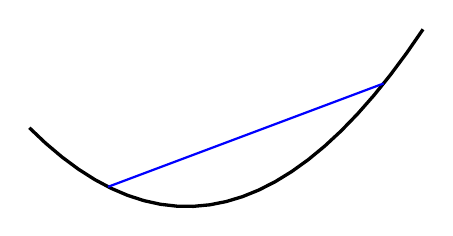
\begin{tikzpicture}
    \draw [domain=-1:4, very thick] plot (\x, {\x*\x/4 - \x/2 - 1});
    \draw [blue, thick] (0,-1) -- (3.5,0.3125);
  \end{tikzpicture}
  \caption{The graph of a convex function under its secant line (blue)}
  \label{fig:convex}
\end{figure}

Although the definition of convex functions only talks about inner division points, it is pleasant to see that this already implies continuity of such functions.
We start with the following lemma.

\begin{lem}
  Let $f : I \to \mathbb{R}$ be a convex function on an interval $I \subseteq \mathbb{R}$.
  Then
  \[
    \frac{ f(x) - f(y) }{ x - y } \leqslant \frac{ f(x) - f(z) }{ x - z } \leqslant \frac{ f(y) - f(z) }{ y - z }
  \]
  for any triplets $x, y, z \in I$ with $x < y < z$.
\end{lem}

The validity of this lemma is clear from Figure~\ref{fig:convex-secant}, when we regard all the fractions as {\em slopes} of the secant lines determined by points on the graph.
The algebraic demonstration of the above inequalities is left to the readers.

\begin{figure}
  \centering
  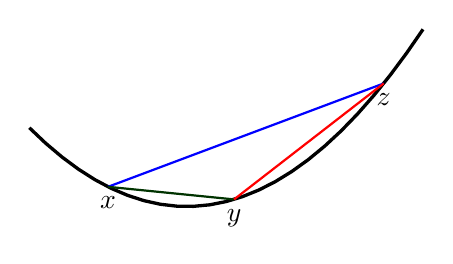
\begin{tikzpicture}
    \draw [domain=-1:4, very thick] plot (\x, {\x*\x/4 - \x/2 - 1});
    \draw [blue, thick] (0,-1) coordinate (X) -- (3.5,0.3125) coordinate (Z);
    \draw [green!20!black, thick] (X) -- (1.6, -1.16) coordinate (Y);
    \draw [red, thick] (Y) -- (Z);
    \node [below] at (X) {$x$};
    \node [below] at (Y) {$y$};
    \node [below] at (Z) {$z$};
  \end{tikzpicture}
  \caption{Comparison of slopes of secant lines on the graph of a convex function}
  \label{fig:convex-secant}
\end{figure}
\begin{thm}
  Let $I$ be a nondegenerate interval in $\mathbb{R}$, and $f : I \to \mathbb{R}$ be a convex function.
  \begin{enumerate}[$(a)$]
    \item For any $x,y$ in $I$ and $s, t \in \mathbb{R}$ with $s + t = 1$ but $s, t \notin [0,1]$, we have
      \[
	f(sx + ty) \geqslant s \, f(x) + t \, f(y), \qquad
	\text{if } sx + ty \in I.
      \]

    \item $f$ is continuous at any interior point of $I$.
  \end{enumerate}
\end{thm}

\begin{proof}
  \begin{enumerate}[$(a)$]
    \item Let $z = sx + ty$.
      By symmetry let us assume that $s < 0$ and $t > 1$.
      Then $y = \dfrac1t z - \dfrac{s}{t} x$ becomes an inner division point of $z$ and $x$ in $I$.
      From the definition of convex functions, we have
      \[
	f(y) \leqslant \frac{1}{t} f(z) - \frac{s}{t} f(x),
      \]
      which is equivalent to $f(z) = f(sx+ty) \geqslant s \, f(x) + t \, f(y)$.

    \item Let $z$ be any interior point of $I$, and fix two points $x,y \in I$ with $x < z < y$.

      Assume first that $t \in I$ and $x < t < z$.  By the definition of convex functions and (1), we have
      \begin{equation}
	\label{ineq:convex1}
	f(z) + \frac{f(x)-f(z)}{x-z} (t-z) \leqslant f(t) \leqslant
	f(z) + \frac{f(y)-f(z)}{y-z} (t-z),
      \end{equation}
      since $t$ is an inner division point of $x,z$ but an outer division point of $y,z$.  By squeeze theorem and (\ref{ineq:convex1}) we see that $f(t) \to f(z)$ as $t \to z-$.

      On the other hand, let us take $t \in I$ and $z < y < t$.
      This time the inequalities (\ref{ineq:convex1}) are reversed:
      \begin{equation}
	\label{ineq:convex2}
	f(z) + \frac{f(x)-f(z)}{x-z} (t-z) \geqslant f(t) \geqslant
	f(z) + \frac{f(y)-f(z)}{y-z} (t-z).
      \end{equation}
      Therefore $f(t) \to f(z)$ as $t \to z+$ as well,
      Since $f(z-) = f(z) = f(z+)$, we conclude that the convex function $f$ is continuous at the interior point $z$ of $I$.
  \end{enumerate}
\end{proof}

\noindent{\em Remark.}
There are a few more properties of convex functions that are related to differentiation.
They will be discussed in the later topics.
\end{document}
